% Chapter 1

\chapter{Background Theory} % Main chapter title

\label{Chapter1} % For referencing the chapter elsewhere, use \ref{Chapter1} 

%----------------------------------------------------------------------------------------

% Define some commands to keep the formatting separated from the content 
\newcommand{\keyword}[1]{\textbf{#1}}
\newcommand{\tabhead}[1]{\textbf{#1}}
\newcommand{\code}[1]{\texttt{#1}}
\newcommand{\file}[1]{\texttt{\bfseries#1}}
\newcommand{\option}[1]{\texttt{\itshape#1}}

%----------------------------------------------------------------------------------------

\section{Artificial Neural Networks}
Artificial neural networks are parallel distributed processing systems that are composed by  neurons, their most elementary building block. Neurons are processing  units that generate an output according to an activation function $\sigma(x)$, which is usually a sigmoid function like in equations \ref{eq:1} and \ref{eq:2}.\\

Logistic Regression: 

\begin{equation}\label{eq:1}
\sigma(h)= \left\{
			 \begin{array}{ll}
			 	1, h\geq0\\
			 	0, h<0
			\end{array}
		 \right.
\end{equation}


Hyperbolic tangent function:

\begin{equation}\label{eq:2}
\sigma(h)=tanh(h)
\end{equation}
\\

Neurons are interconnected by links, which have strengths that are coded by weights. A zero weight for example would indicate that absence of connection between two neurons. The link weights can also be tuned based on experience, an important property that makes neural networks adaptable and trainable. 
\\
Figure~\ref{fig:Neuron} shows a mathematical model of a neuron based on [\cite{Reference2}], with $n$ input signals $x_1, x_2, ..., x_{n}$ and an output signal $y$. This model also shows the weights of each of the input links of this neuron as $w_1, w_2,...,w_{n} $, a bias term $w_0$ and an activation function $\sigma(.)$. In this model $x_0$ is equals to $1$ to include the bias term within the same vector form. 
\\
The output of this neuron is the aggregation of the input signals, shifted by the bias term and processed by the activation function; as shown in equation \ref{eq:3}.

\begin{figure}[h]
	\centering
	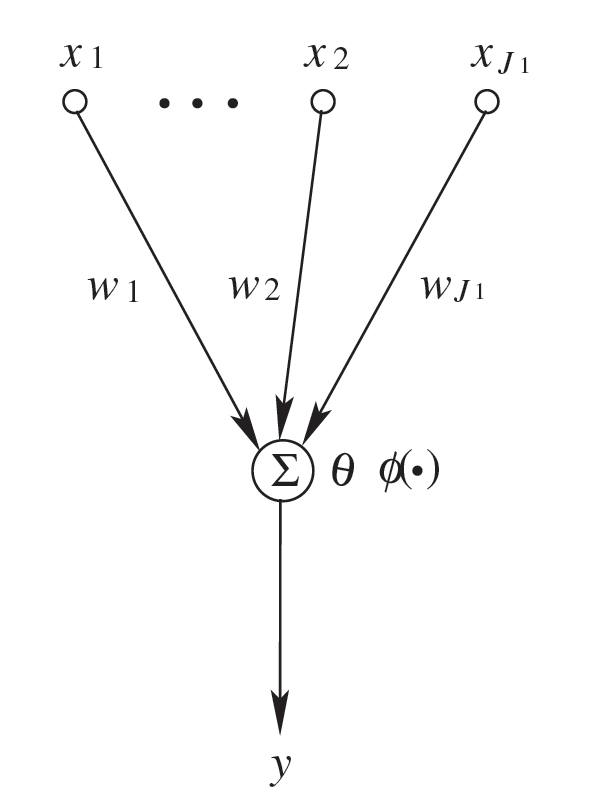
\includegraphics{Figures/neuron_mathematical_model.PNG}
	\decoRule
	\caption[Mathematical Model of a Neuron]{Mathematical Model of a Neuron.}
	\label{fig:Neuron}
\end{figure}

\begin{equation}\label{eq:3}
	y=\sigma(input + bias)=\sigma(W^{T}X)=\sigma(\sum_{i=0}^{n} w_i x_i)
\end{equation}
\\
\subsection{Types of Neural Networks}
The arrangement of synaptic links between neurons determines different types of neural networks. If the links are acyclic for example, the neural network is considered a FNN; while the presence of cyclic links indicates a RNN. The understanding FNNs is essential to the understanding of RNNs, so a more detailed description of training and characteristics of FNNs is given in Appendix \ref{AppendixA}. 
%----------------------------------------------------------------------------------------





\section{Recurrent Neural Networks}
Neural Networks with cyclic links are considered RNNs.
\\\\
\textcolor{red} {[TODO: Introduce general idea of RNNs] }
\section{Training RNNs}

\subsection{Backpropagation Through Time}
BPTT is an adaption of the backpropagation method used in FNNs.

\section{Challenges in RNNs}
It has been theoretically proven that RNNs can be universal approximators of dynamic processes [\cite{Reference1}], which represents a powerful potential for modeling natural systems more accurately compared to existing methods such as FNNs. However, practical applications of RNNs have been stagnated due to theoretical and implementation challenges encountered in the this model. This section specifies some of these challenges. 

\subsection{Computational Cost}

\textcolor{red} {[TODO: Expand!] }
%High computational cost for non-linear activation functions such as sigmoid functions.

\subsection{Supervised Training}

\textcolor{red} {[TODO: Expand!] }


%----------------------------------------------------------------------------------------

